\section{Evaluation} \label{sec:evaluation}
SECTION NOT YET UPDATED. Not worth proofreading yet. 

We will now demonstrate the scalability of the supersets encoding scheme table size for a real exchange point. 

\subsection{Experimental Setup}
We used a data set from the AMS-IX exchange point~\cite{ams-ix}, which gave us access to 63 participants advertising over 600,000 prefixes. Although not on the scale of complete data sets of the largest exchange points, the data set is large enough that the partial masks optimization is required to fit masks into the MAC field. Our experiments were run on a laptop with a 4-core CPU running at 2.4GHz and 16GB of RAM.

The exchange point considered does not yet have support for SDN forwarding rules, so instead we simulate the number of forwarding entries required by the outbound policy of a hypothetical participant which is able to see all available route announcements. The participant was given 1000 uniformly random forwarding entries to a uniformly random subset of participants, with each subset size corresponding to a different experiment. 

\subsection{Performance}
We run our evaluations against a RIB dump of AMS-IX retrieved on May 1st, 2016 from the RIPE Routing Information Service raw data webpage~\cite{ris}.

\begin{figure}[t!] 
\begin{minipage}{1\linewidth}
\begin{subfigure}[b]{0.96\linewidth}
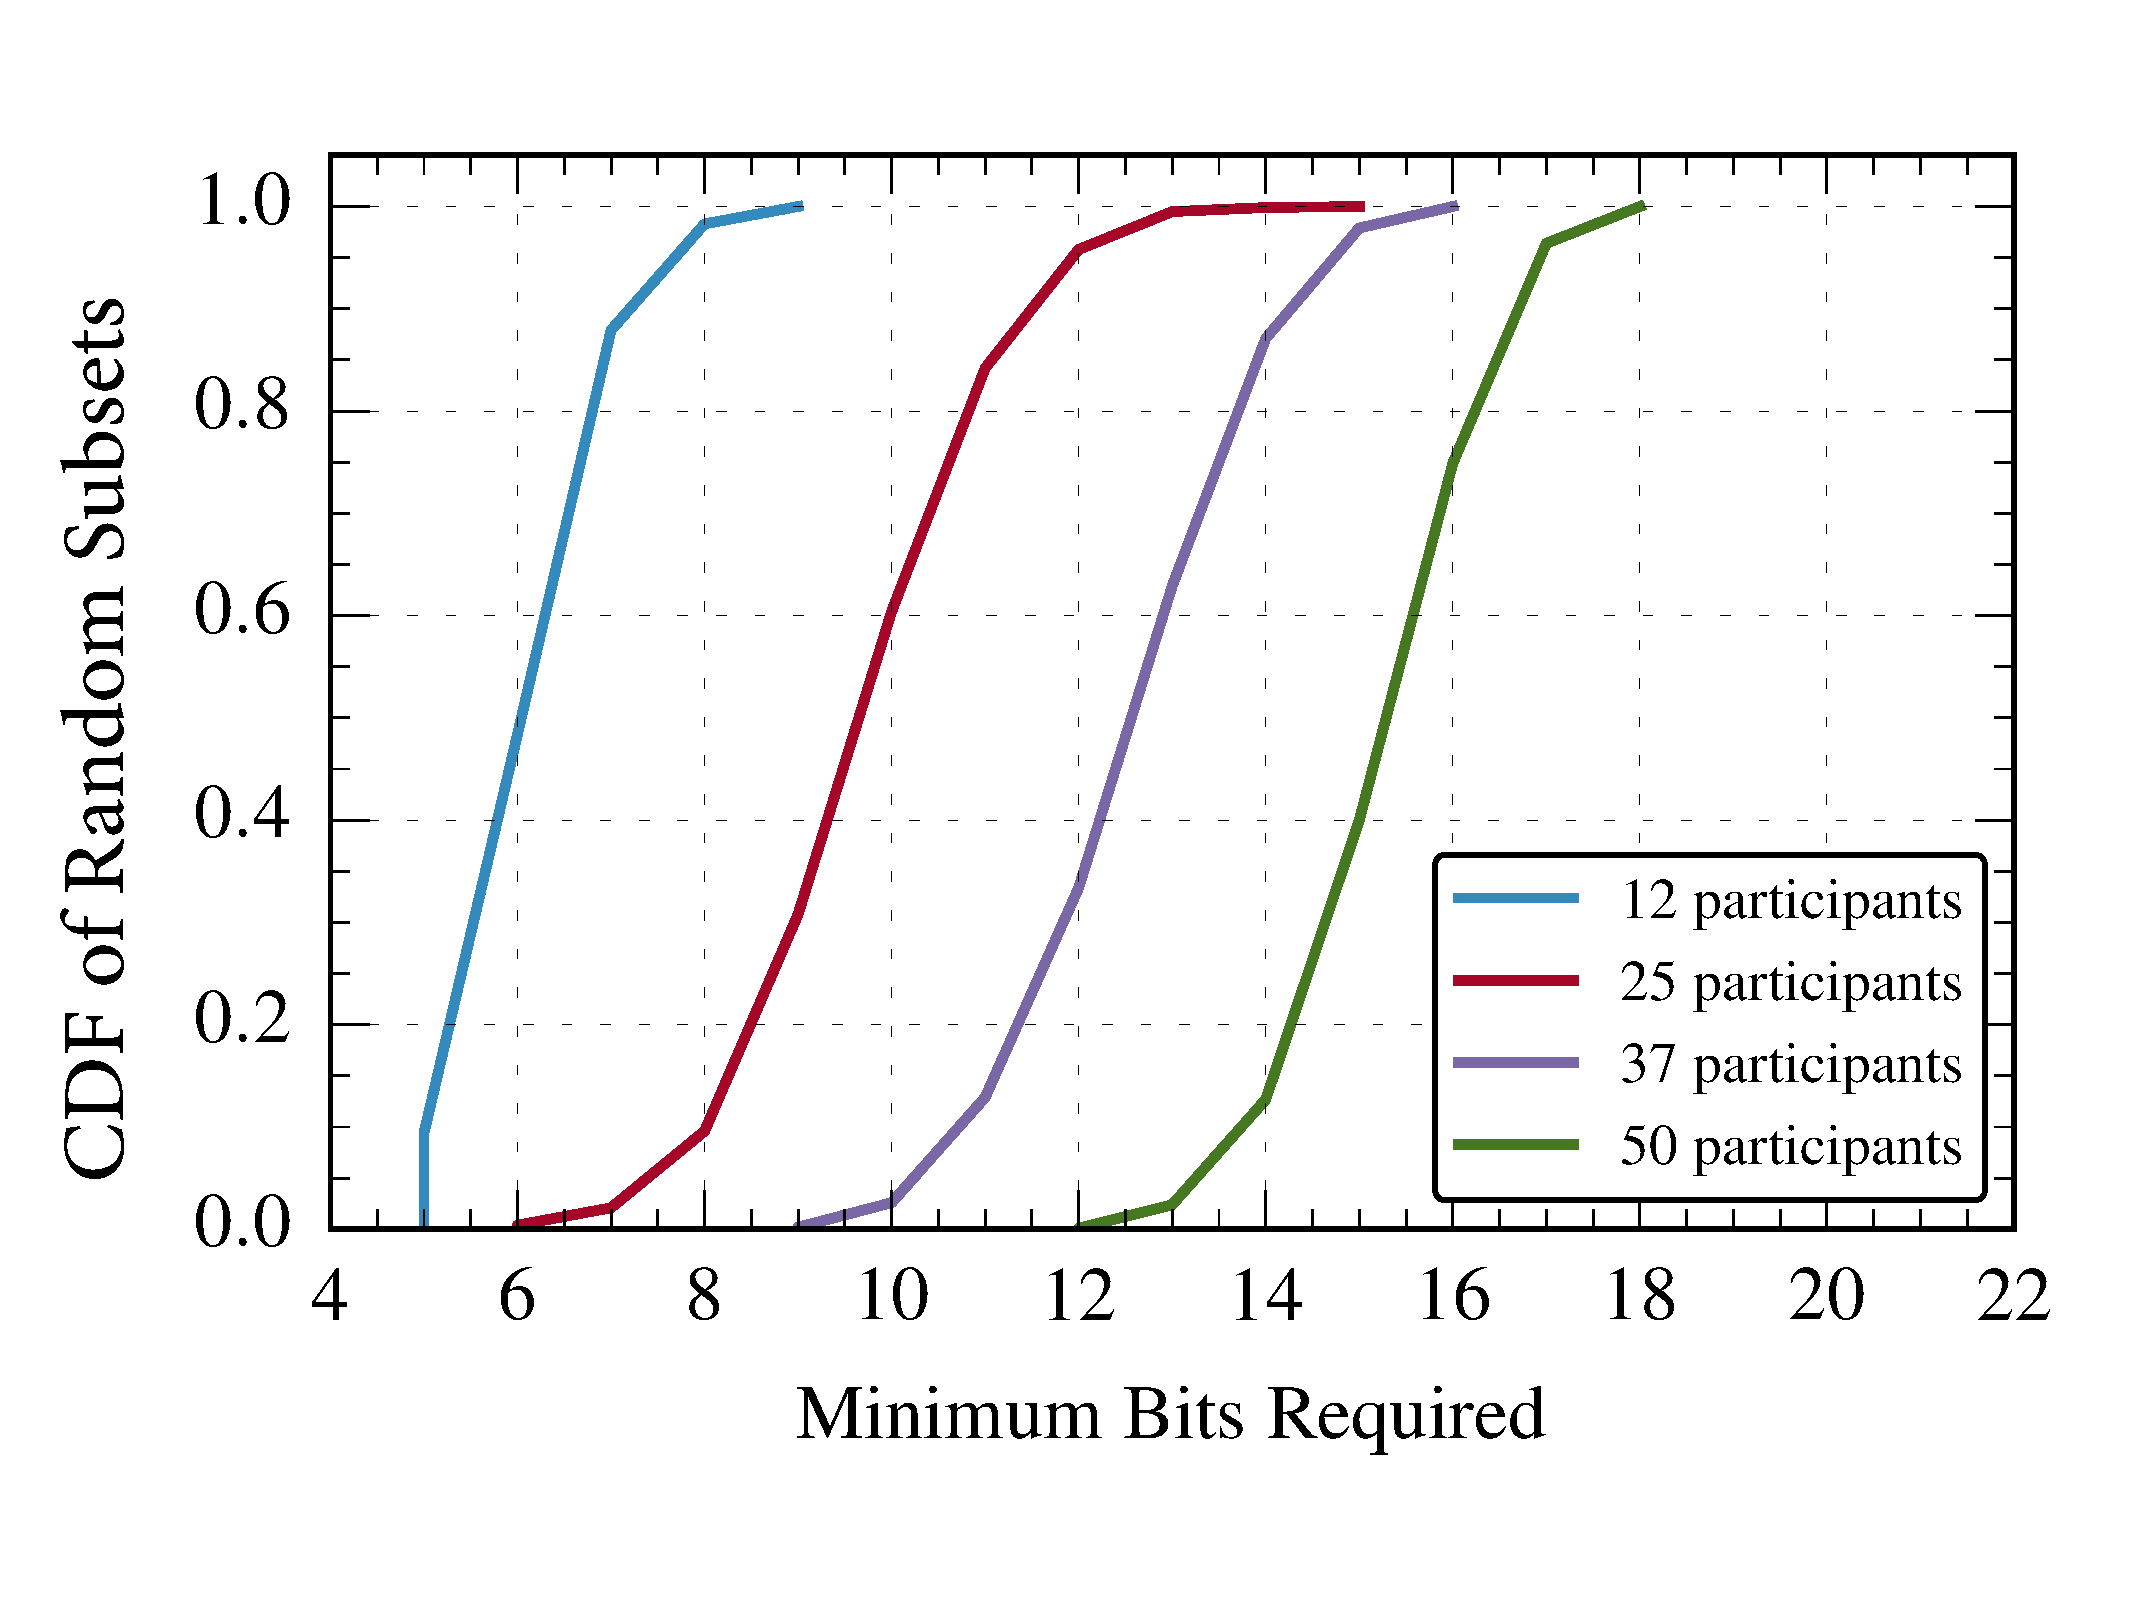
\includegraphics[width=\linewidth]{figures/bit_counts}
\end{subfigure} 
\end{minipage} 
\caption{Minimum number of bits required by a feasible solution for a random policy which forwards to a random subset of participants.}
\label{fig:bits}
\end{figure}

In order for our encoding scheme to successfully work, it must compress the information to the point that it fits into the MAC address field, which is restricted to 48 bits if no other information is encoded alongside reachability. Figure \ref{fig:bits} shows the number of bits required by our reachability encoding with uniformly randomly chosen active sets, repeated 500 times for each active set size. In the worst case, 18 bits were required when considering all 63 participants. The graphs appear to show that the number of bits required scales linearly with the number of participants present in the active set. However, we believe that the number of bits required actually scales sublinearly with the size of the active set, and that the appearance of linear scaling is a consequence of our simulation method. In order for the bits required to scale linearly, the number of participants that simultaneously advertise a single precept would have to also increase linearly in the size of the IXP, but we suspect this is not the case. Even if the number of bits required were indeed to scale linearly, extrapolating out the graph yields that, in the worst case, a participant's active set could contain over 100 participants, allowing very complex forwarding policies.

\begin{figure}[t!] 
\begin{minipage}{1\linewidth}
\begin{subfigure}[b]{0.96\linewidth}
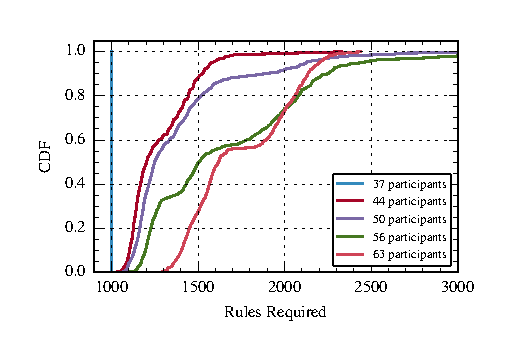
\includegraphics[width=\linewidth]{figures/rule_cdf}
\end{subfigure} 
\end{minipage} 
\caption{Number of rules required after encoding for a random policy of 1000 rules to random subsets of participants.}
\label{fig:rules}
\end{figure}

Figure \ref{fig:rules} shows the number of rules required by our encoding scheme after running the greedy algorithm with a bit limit of 37, allowing 11 bits for the ``mini-MAC". In this experiment, we began with a baseline policy of 1000 rules, with each rule forwarding to a participant chosen uniformly at random from a random active set. The experiment was repeated 500 times for each active set size, and the number of rules required after applying our encoding was plotted. When the active set is of size 37 or fewer, all participants can fit into a single mask, resulting in zero rule inflation. For active sets of size greater than 37, we can see that the inflation factor is at most 2 in the average case and 3 in the worst case for all active sets. 


\begin{figure}[t!] 
\begin{minipage}{1\linewidth}
\begin{subfigure}[b]{0.96\linewidth}
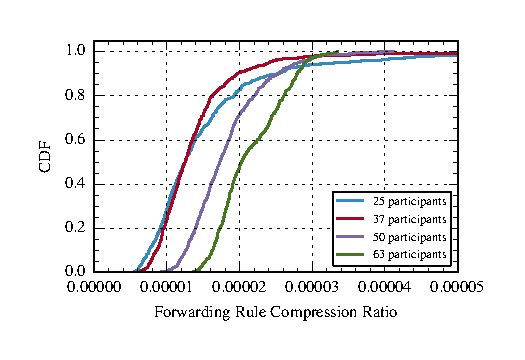
\includegraphics[width=\linewidth]{figures/compression_cdf}
\end{subfigure} 
\end{minipage} 
\caption{Ratio of flow rules required by our encoding algorithm versus the uncompressed
case on random policies involving random subsets of participants.}
\label{fig:compression}
\end{figure}

Figure \ref{fig:compression} shows how the number of flow rules generated by our approach compares to the naive case of zero compression. The compression ratio of our approach versus the naive approach is 20,000 to 1 in the worst case for all active set sizes, and 50,000 to 1 in the median case.


\begin{figure}[t!] 
\begin{minipage}{1\linewidth}
\begin{subfigure}[b]{0.96\linewidth}
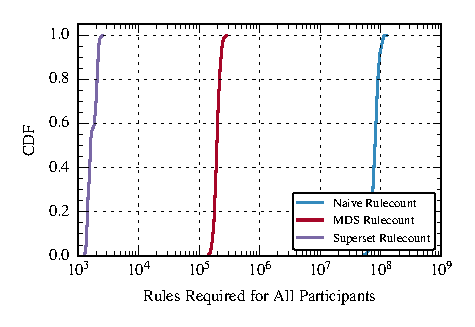
\includegraphics[width=\linewidth]{figures/comparison_cdf}
\end{subfigure} 
\end{minipage} 
\caption{Comparison of the number of flow rules required by our encoding algorithm to the previous state-of-the-art MDS encoding algorithm and the uncompressed case for a random policy involving all participants.}
\label{fig:comparison}
\end{figure}


Figure \ref{fig:comparison} compares our approach to the uncompressed case, as well as to the previous state-of-the-art, the MDS algorithm used in the original SDX system~\cite{sdx}. The comparisons were made using the same approach of generating 1000 random rules, except for the MDS simulation. The MDS algorithm requires each prefix's default next-hop as part of the input, so in each trial we chose next-hops uniformly at random from the list of available next-hops. The graph shows that our approach consistently compresses the number of flow rules by two orders of mangitude greater than the MDS algorithm, which itself compressed the number of flow rules required by the naive case by three orders of magnitude. 

\begin{figure}[t!] 
\begin{minipage}{1\linewidth}
\begin{subfigure}[b]{\linewidth}
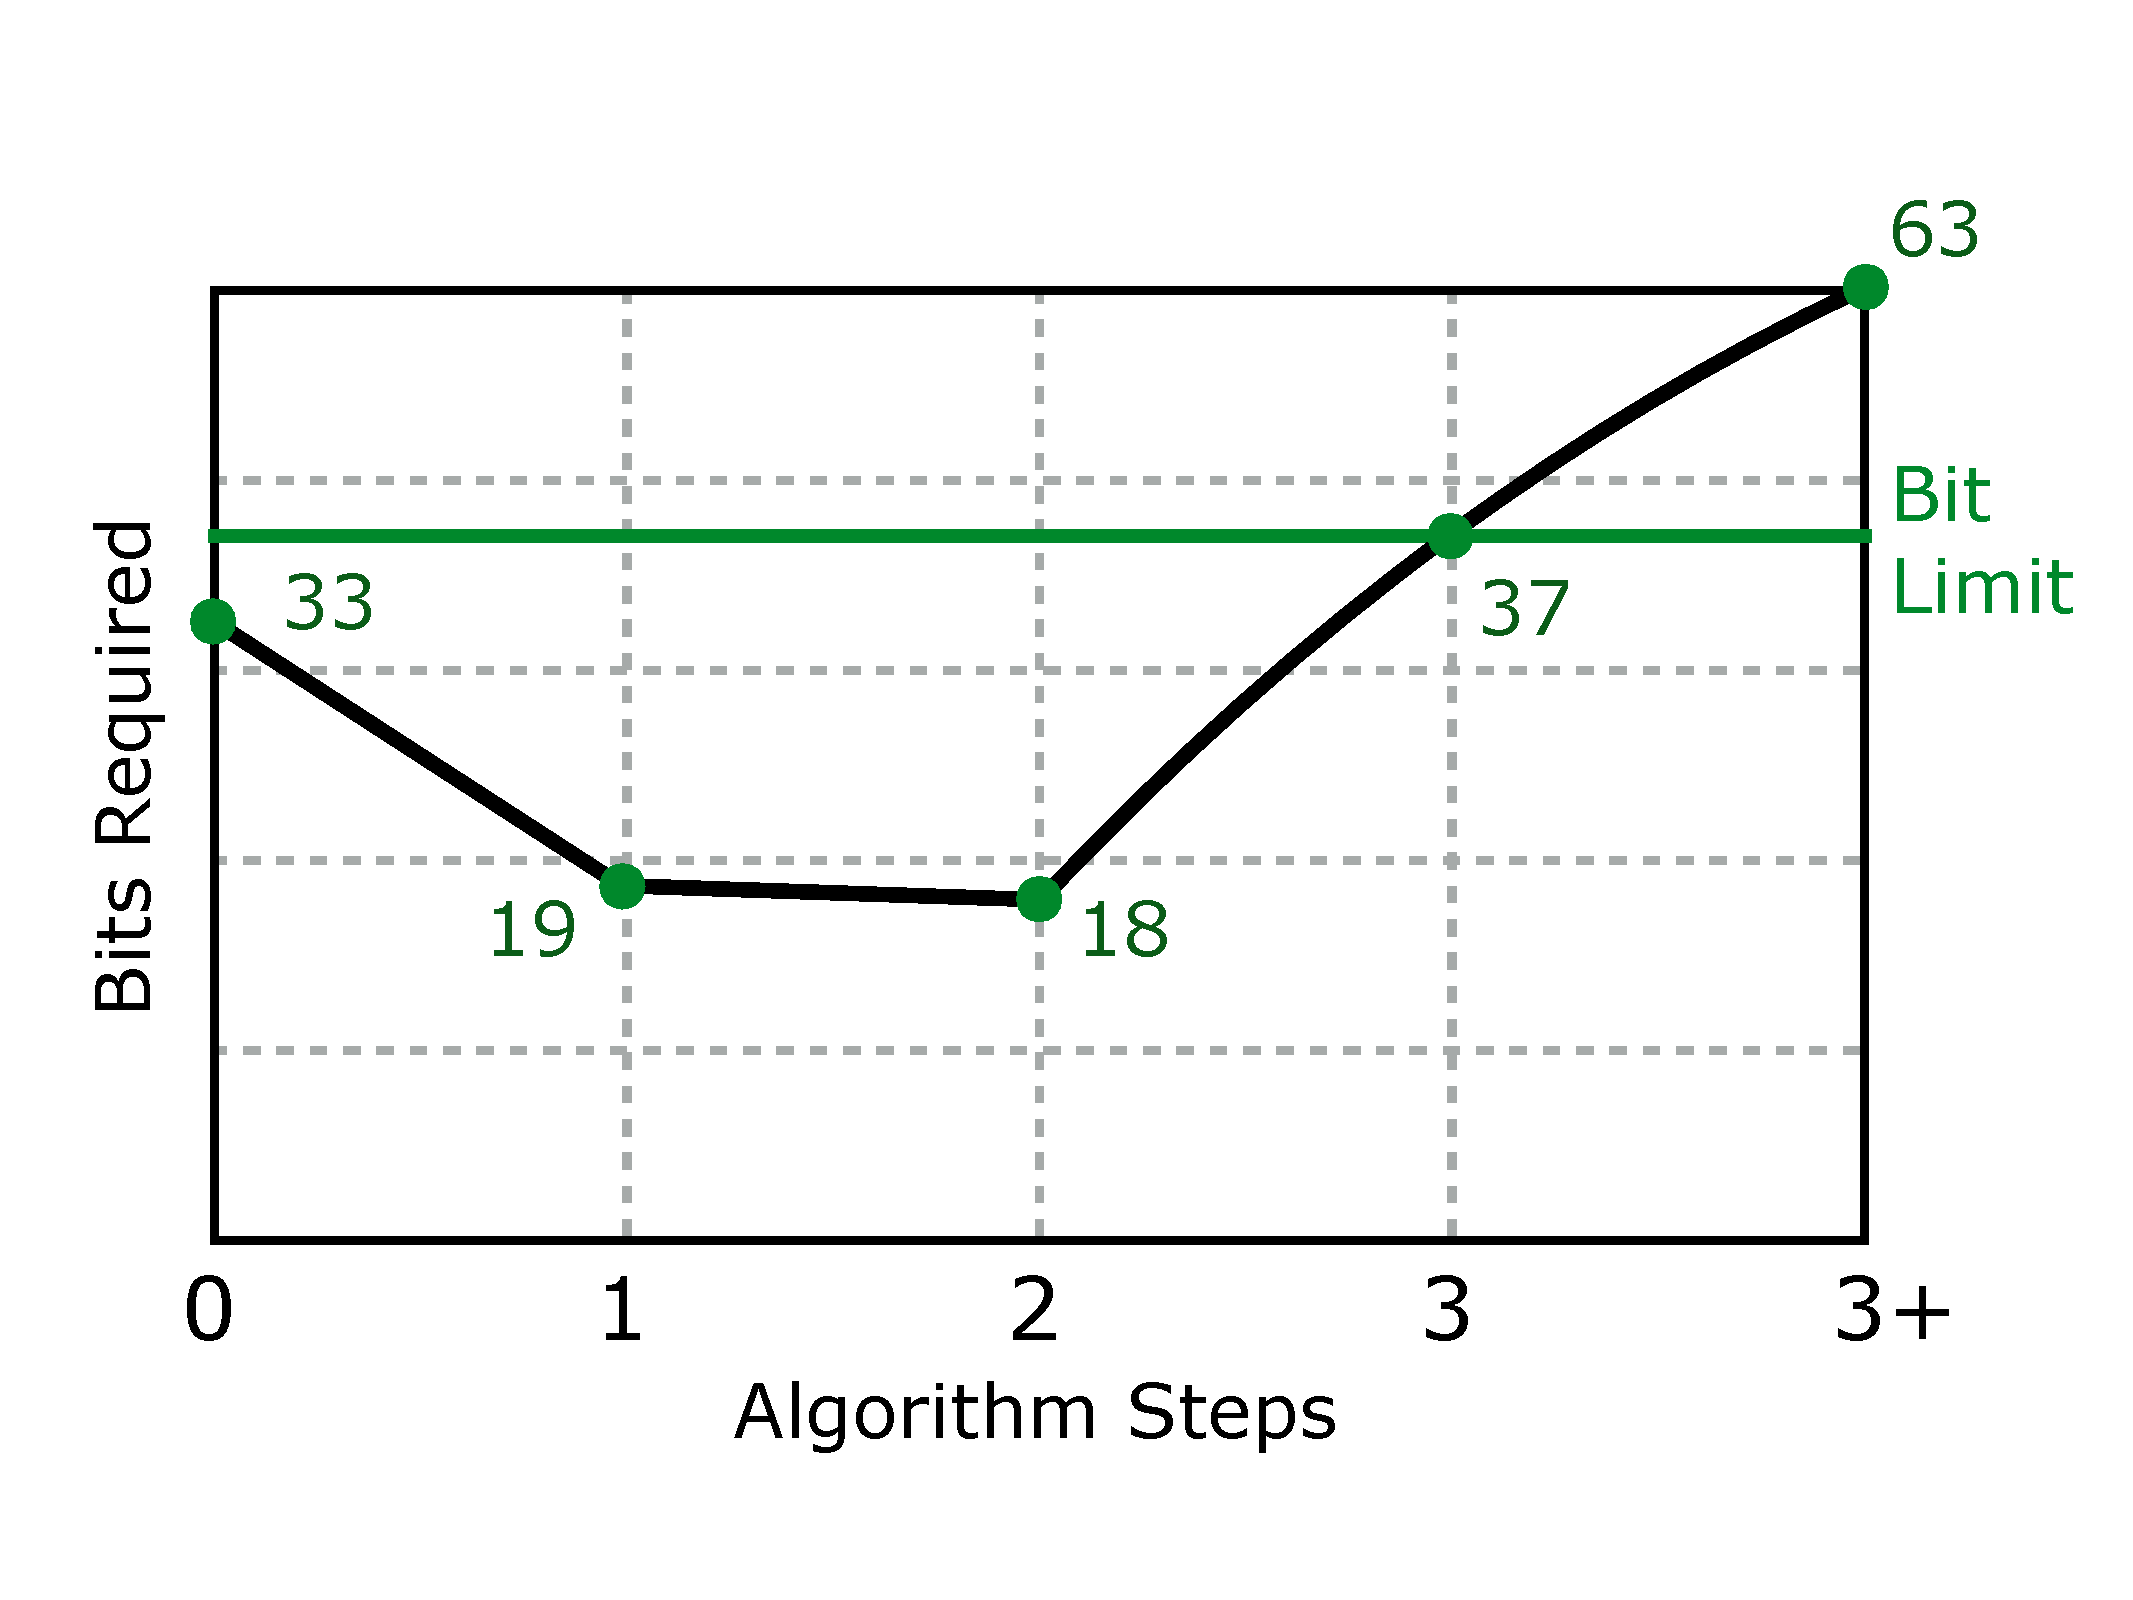
\includegraphics[width=\linewidth]{figures/bit_graph}
\end{subfigure} 
\end{minipage} 
\caption{Graph of the number of bits required by the encoding scheme at each step of the algorithm, shown with real values computed over the AMS-IX RIPE data set. Step 0 is the input of all sets, step 1 is removal of subsets, step 2 is attempting greedy bit minimization, step 3 is after greedily decreasing inflation up to the bit limit, and step 3+ is with no bit limit. }
\label{fig:bit_graph}
\end{figure}